\chapter{Constrained ICA}
\label{ch:constrained_ica}

As discussed in previous chapters, Independent Component Analysis is a standard algorithm for Blind Source Separation. The term blind refers to the fact that the algorithm has no prior knowledge of the mixing matrix $\mathbf{A}$ or the original sources. This means that this method attempts to recover the original sources by only using the statistical properties of the observed mixtures. 

Therefore, the purpose of this chapter is to revisit ICA and study whether adding physiological information or additional knowledge about the separation problem can improve source separation in those cases where standard ICA fails.

\section{Principle}

In Section \ref{sec:ica_derivation}, ICA was described as a sequence of geometrical transformations. As explained in such section, the main difficulty appears after whitening, when the data $Z$ has already been decorrelated and normalized, but still in need of one last final rotation. For this reason, ICA is commonly formulated as an optimization problem, where the objective is function is an estimator of non-Gaussianity, such as kurtosis or negentropy (FastICA). 

\begin{equation}
\theta^\star = \arg\max_{\theta} J\left(\mathbf{y}(\theta)\right)
\end{equation}

However, since non-Gaussianity is computed using higher order statistics, ICA generally becomes a \textbf{non-convex optimization problem}. As a result, the algorithm may converge to different optima due to the initialization, preprocessing and noise level interference \cite{trehan_non-convex_2020,danilova_recent_2022}. In the weak-source problem considered for this thesis, this is especially important, since the component that best satisfies ICA objective function may correspond to the dominant source $s_2$, not the target source $s_1$. 

For this reason, when $s_1$ and $s_2$ are not easily separable through the standard ICA rotation, it may be useful to guide the optimization towards a specific local optimum. This can be achieved by introducing constraints that restrict the feasible region and guide the solution to converge towards a component that is more physiologically meaningful for the target source $s_1$. Equation \ref{eq:constrained_standard_form} shows the mathematical representation of this idea, where each function $g_i$ defines a constraint that limits the feasible region.

\begin{equation}
\begin{array}{ll}
    \underset{\theta}{\mathrm{maximize}} 
    & J\left(\mathbf{y}(\theta)\right) \\[0.2cm]
    \mathrm{subject\ to} 
    & g_1(\theta) \leq 0 \\
    & g_2(\theta) \leq 0 \\
    & \vdots \\
    & g_n(\theta) \leq 0
\end{array}
\label{eq:constrained_standard_form}
\end{equation}

To further clarify this concept, Figure \ref{fig:constrained_conceptual_graph} visually interpretation of the presented ICA constrained formulation. In the unconstrained case, ICA selects the global maximum of this objective, which in the weak-source model usually corresponds to the dominant source $s_2$. By adding problem related constraints, the feasible region (blue shaded area in graph) can be restricted to a local optimum that is more consistent with the target source $s_1$. 

\begin{figure}[H]
    \centering
    \makebox[\textwidth][c]{%
        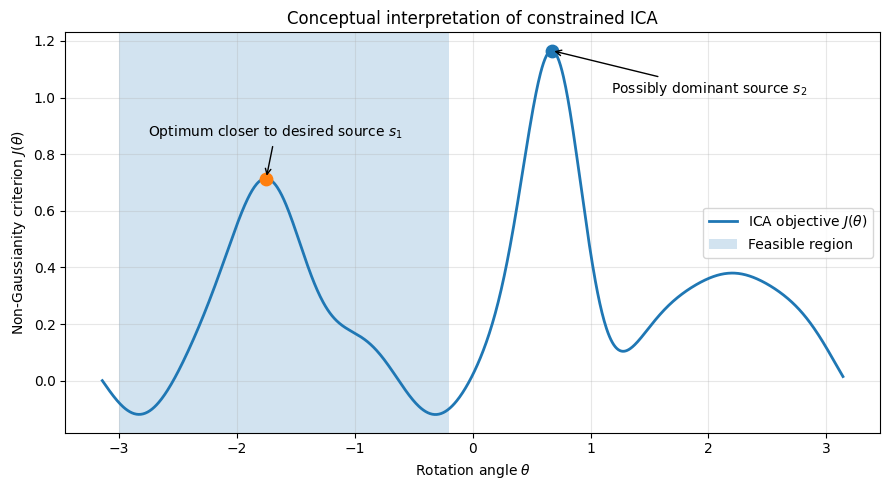
\includegraphics[width=\linewidth]{figuras/constrained_conceptual_graph.png}
    }
    \caption{Conceptual illustration of constrained ICA in weak-source scenario. The curve represents a generic non-Gaussianity objective, not real experimental negentropy values.}
    \label{fig:constrained_conceptual_graph}
\end{figure}


Conceptually, this version of ICA is only expected to improve standard ICA in scenarios where interferences such as noise or delay prevent the orthogonal component from aligning correctly with $s_1$. In these cases, the constraints guide the optimization algorithm towards a optimum that is more aligned with the target source $s_1$, even if this slightly reduces the quality of the recovered dominant source $s_2$. Since the main objective of this thesis is to recover $s_1$ (target flap-related source) this trade-off is acceptable.

\section{Constraints}

The key idea introduced in the previous section is only useful if the added constraints are specifically related to the target source $s_1$. In other words, the constraints must provide information that helps identify $s_1$ from the dominant source $s_2$. This information can either describe expected properties of the signal itself, such as temporal pattern or envelope or knowledge about the separation problem. 


This section aims to present ideas and possibilities for these constraints as well as relevant consideration for their application in the weak-source EMG separation problem.

\subsection{Constraint Examples}
\subsubsection{Spatial constraints}

In high-density EMG studies, such as the TMR dataset used in this thesis \cite{todd_kuiken_electromyography_2023}, information about electrode placement can be valuable because it provides spatial context about the recorded channels. This information may allow the algorithm to consider that signals recorded by nearby electrodes may contain similar sources due to volume conduction or anatomical proximity \cite{hesse_fastica_2005}. Equation \ref{eq:spatial_constraint_example} denotes a simplified spatial constraint example, where the estimated projection $\mathbf{a}_i$ is considered to remain close to a reference topography $\mathbf{a_{c,i}}$. The parameter $\epsilon$ controls the allowed deviation. 
\begin{equation}
    g_i(\mathbf{A})
    =
    \left\|
    \mathbf{a}_i - \mathbf{a}_{c,i}
    \right\|^2
    \leq \epsilon
    \label{eq:spatial_constraint_example}
\end{equation}

However, in the weak-source scenario considered in this work, these constraints may not be helpful since the target source $s_1$ is not necessarily aligned with a dominant spatial projection. Observing the weak-source model in Section \ref{sec:weak_source_regime}, $s_1$ is weakly represented across the electrodes,  which makes defining a reliable reference topography $\mathbf{a}_{c,i}$ becomes considerably difficult. As a result, the spatial constraints could guide the algorithm towards dominant source $s_2$ rather than improving the recovery of $s_1$.

\subsubsection{Temporal constraints}
Temporal constraints introduce prior information about the expected time behavior of the source signals. Instead of guiding the separation through spatial projections, these constraints guide the algorithm based on how the desired component is expected to behave over time \cite{yang_flexible_2025,lu_ica_2006}. This can be useful in EMG when some information about activation pattern of the target source is available, such as reference signals, calibration contractions or expected RMS envelopes. Equation \ref{eq:temporal_constraint_example} denotes a simplified temporal constraint example where $\hat{s}_i$ is the estimated source, $r_i$ the temporal reference with the desired component.

\begin{equation}
    g_i(\mathbf{s})
    =
    \left\|
    \hat{s}_i - r_i
    \right\|_2^2
    \leq \epsilon
    \label{eq:temporal_constraint_example}
\end{equation}

However, for EMG this kind of constraints may become too restrictive in some cases, since the waveform can change due to phase shifts and delays.

\subsubsection{RMS envelope constraints}
In EMG context of this thesis,  RMS envelope constraints can be considered as a less restrictive version of temporal reference constraints. Instead of requiring the estimated source align sample by sample, they compare their RMS envelopes. This is more appropriate for EMG because it focuses on the activation pattern of $s_1$ and is less sensitive to shifts and delays.  Equation \ref{eq:rms_constraint_example} shows this idea mathematically, where the RMS envelope of the estimated source is constrained to remain close to the RMS envelope of the reference signal.


\begin{equation}
    g_i(\mathbf{s})
    =
    \left\|
    \mathrm{RMS}(\hat{s}_i)
    -
    \mathrm{RMS}(r_i)
    \right\|_2^2
    \leq \epsilon
    \label{eq:rms_constraint_example}
\end{equation}

Though this type of constraint may be the best fit for this thesis as its implementation is not trivial. Since the RMS envelope is a nonlinear transformation of the signal, incorporating it directly into the FastICA optimization would considerably complicate the update rule. This would likely require a redesign of the algorithm rather than modification of the existing fixed-point iteration.


\subsubsection{Considerations}

One final consideration is that the constraints \textbf{must be expressed as functions of the optimization variable} (rotation angle $\theta$ or the separation vector $\mathbf{w}$). Even if they are initially defined in terms of source properties, spatial projections or RMS envelopes, they must ultimately be linked to the variable being optimized so that they can modify or restrict the ICA solution. This point will be especially relevant in Section \ref{sec:constrained_ica_implementation}.

\subsection{Constraint strength}

Given a specific separation problem, there may occasions were some constraints are required to be met, while others may be met partially. Therefore, it is important to distinguish between two types:

\subsubsection{Hard constraints}

These constraints impose conditions that must be strictly satisfied. Mathematically, constraints are usually represented as functions of the decision variable that must be equal to zero or less than or equal to zero.

\[
\max_{\theta} J(\theta)
\quad \text{s.t.} \quad
g_i(\theta) \leq 0
\]
In real world scenarios, these constraints may become problematic sometimes because an inaccurate or overly restrictive constraint can potentially make the optimization infeasible. In other words, there may be no solution that satisfies all imposed conditions while still optimizing the ICA objective.


\subsubsection{Soft constraints}
These constraints can be partially met in case an objective optimum requires it. This means they allow some deviation and can be mathematically represented as a penalty term that is added to the objective function. 

\[
    \max_{\theta}
    \left[
    J(\theta) - \lambda g_i(\theta)
    \right]
\]
where $\lambda$ controls the weight of the constraint. Larger values of $\lambda$ force the solution to satisfy the constraint more strongly and when $\lambda \rightarrow \infty$ it can understood as a hard constraint.
\section{Implementation}
\label{sec:constrained_ica_implementation}

Since this approach is tailored to specific separation problems and depends on the type of prior information available, \uline{there is no standardized library function for constrained ICA} in the same way there is for conventional FastICA. For this reason, the main objective of this section is to describe which constraints can be considered viable for this work and how they can be added into the fixed-point iteration.


In specific, this implementation focuses on \textbf{soft reference constraints}, where standard fixed point update is not replaced. Instead, it is guided using constraint information related to the \uline{target source and dominant source}.

To impose the soft constraints and modify the fixed point update, the reference signal must first be transformed into a direction in the whitened space  \cite{wang_fixed-point_2011}. This allows the temporal information contained in the reference to be expressed in terms of the optimization variable $\mathbf{w}$ (can also be expressed in terms of $\theta$). Equation \ref{eq:reference_direction} shows this transformation, where the reference direction is computed from the correlation between the whitened data $\mathbf{z}$ and reference signal $r$.
\begin{equation}
\mathbf{q}(\tau)
=
\mathbb{E}\left[\mathbf{z}(t) r(t-\tau)\right]
\label{eq:reference_direction}
\end{equation}

Since the magnitude of this vector depends on the scale of the reference signal and the strength of its correlation, it has to be normalized before being used in the update rule. This guarantees that $\mathbf{q}$ only represents a direction in the whitened space. 

\begin{equation}
\mathbf{q}
=
\frac{\mathbf{q}(\tau^\star)}
{\left\|\mathbf{q}(\tau^\star)\right\|}
\end{equation}

This idea is implemented in $\texttt{BuildReferenceDirection}$ function which can be found in \textbf{Appendix \ref{app:build_reference_direction}	}.

After transforming the reference into a suitable direction, the fixed point update is extended with two extra steps. The positive correction term is derived soft constraint that \textbf{rewards} alignment between $\mathbf{w}$ and $\mathbf{q}_{target}$. This can be measured using the scalar product $\mathbf{w}^T\mathbf{q}_{target}$, which leaves the corresponding objective term as shown in Equation \ref{eq:positive_soft_constraint}.

\begin{equation}
\lambda_{pos}
\left(
\mathbf{w}^{T}\mathbf{q}_{target}
\right)^2
\label{eq:positive_soft_constraint}
\end{equation}

After this, taking the gradient of the term with respect $\mathbf{w}$ gives the correction applied to the fixed point update.

\begin{equation}
\Delta \mathbf{w}_{target}
=
2\lambda_{pos}
\left(
\mathbf{w}^{T}\mathbf{q}_{target}
\right)
\mathbf{q}_{target}
\label{eq:positive_correction}
\end{equation}
where $\lambda_{pos}$ controls the weight of the correction towards the target reference. By contrast, the negative correction term is derived in a similar way, but by \textbf{penalizing} the dominant direction. 

\begin{equation}
\lambda_{neg}
\left(
\mathbf{w}^{T}\mathbf{q}_{bad}
\right)^2
\label{eq:negative_soft_constraint}
\end{equation}
where $\lambda_{neg}$ controls how strongly the solution avoid the undesired direction. Overall, the complete update can be seen as shown in Equation \ref{eq:constrained_fastica_update}. 

\begin{equation}
\mathbf{w}
\leftarrow
\operatorname{FixedPointUpdate}(\mathbf{w})
+
\Delta \mathbf{w}_{target}
-
\Delta \mathbf{w}_{bad}
\label{eq:constrained_fastica_update}
\end{equation}



Theoretically, the main advantage of this implementation is that the weights of each reference can be adjusted based on the confidence. If a reference is considered reliable, its corresponding weight can be increased so that the algorithm follows that information more strongly. By contrast, if a reference is only an approximate of the desired activation pattern, a lower weight can be used, which approaches the method to the standard FastICA.

Taking all the mentioned considerations into account, the constrained ICA algorithm can be structured in a similar way to the traditional FastICA implementation described in Section \ref{sec:ica_implementation}. The main difference is the introduction of an additional step to include the reference directions before the fixed point iteration begins. 

\begin{itemize}
    \item \textbf{Preprocessing:} same idea as in FastICA (for more preprocessing detail refer to Chapter \ref{ch:preprocessing}).
    \item \textbf{Build reference direction: }before starting fixed point iteration, references must be transformed into directions in the whitened space.  
    \item \textbf{Fixed point update: }this update adds the two weighted reference terms to the original FastICA fixed point update.
    \item \textbf{Ensure convergence: }at the end of each iteration, it is necessary to normalize the $\mathbf{w}$ term to guarantee the convergence of the algorithm.
    
\end{itemize}

Listing \ref{lst:constrained_fastica_pseudocode} illustrates the constrained ICA pseudocode of the implementation designed for this thesis.

\clearpage

\begin{lstlisting}[
style=pseudocode,
caption={Reference-constrained FastICA},
label={lst:constrained_fastica_pseudocode},
escapeinside={(*@}{@*)}
]
Input: Observed EMG matrix X, target reference r_target,
       interference reference r_bad, constraint weights lambda_pos,
       lambda_neg, tolerance epsilon, maximum iterations Imax

Output: Estimated target source y_hat and separation vector w

//Preprocessing
Xc <- X - mean(X)
Z  <- Whiten(Xc)

//Reference directions
q_target <- ReferenceDirection(Z, r_target)
q_bad    <- ReferenceDirection(Z, r_bad)
//Initialization
w <- Initialize(q_target)
w <- Normalize(w)
//Constrained optimization
for i = 1 to Imax

    w_old <- w
    w <- FastICAUpdate(w, Z, g)
    w <- w + (*@$\Delta \mathbf{w}_{target}$@*)
    w <- w - (*@$\Delta \mathbf{w}_{bad}$@*)
    delta <- | |w * w_old^T| - 1 |
    if delta < epsilon
        break
    end

end

y_hat <- Xc * w

return y_hat, w
\end{lstlisting}

However, \uline{this implementation does not guarantee an improvement over the traditional ICA}, especially if the reference does not provide valuable information about $s_1$ non-Gaussianity. In real world scenarios, the best reference that would be available for the weak source would at most be a binary mask of the target muscle activation.
\clearpage


\section{Baseline comparison: Linear Regression}


Before evaluating the proposed constrained ICA approach, it is useful to consider a simpler baseline  to compare constrained ICA with other algorithms that use references or prior information. In the specific case where the second observed channel can be interpreted as an approximate reference of the dominant source (model in Equation \ref{eq:weak_noise_model}), the recovery of the weak source can be expressed as an interference cancellation problem. This theoretically enables the use of the classic linear regression algorithms to estimate the contribution of the reference channel $c_2$ in the contaminated $c_1$ \cite{samaniego_separation_1997}.

Recalling the weak source model explained in Section \ref{sec:weak_source_regime} ($\tau=0$), channel $c_1$ is defined as $s_1$ with a contamination from $s_2$ and additive noise.

\begin{equation}
    c_1(t) = s_1(t) + \beta s_2(t) + n_1(t),
\end{equation}

Assuming that $c_2$ provides an approximate observation of the interfering component $s_2$, a linear estimate of the contamination in $c_1$ can be obtained by projecting $c_1$ onto $c_2$. The regression coefficient is therefore computed as shown in Equation \ref{eq:regression_beta}.

\begin{equation}
    \hat{\beta} =
    \frac{\mathbf{c}_2^T \mathbf{c}_1}
    {\mathbf{c}_2^T \mathbf{c}_2}.
    \label{eq:regression_beta}
\end{equation}

The estimated weak source is then obtained by subtracting this contribution from the first observed channel:

\begin{equation}
    \hat{s}_1^{\mathrm{reg}}(t) =
    c_1(t) - \hat{\beta}c_2(t)
    \label{eq:regression_s1}
\end{equation}

This approach is computationally simple and does not require an iterative optimization algorithms. However, it relies on the assumption that $c_2$ is an accurate reference of the dominant source. In the model considered in this thesis, $s_2$ may be dominant in $c_2$, but it also contains noise and small contribution from the target source $s_1$.

\begin{equation}
    c_2(t) = 0.01s_1(t-\tau) + s_2(t) + n_2(t),
\end{equation}

Therefore, standard linear regression is not expected to provide an ideal recovery of $s_1$, but it represents an important baseline for evaluating whether the added complexity of constrained ICA produces a meaningful improvement. One final note is that, unlike the previously mentioned separation algorithms, linear regression can better estimate the original scale of $s_1$, but its accuracy depends on the contamination in $c_2$. 

Alternatively, if delay is accurately estimated, a modified version of linear regression can be rewritten. 

\begin{equation}
    \hat{\beta} =
    \frac{\mathbf{c}_2^T(t-\tau) \mathbf{c}_1}
    {\mathbf{c}_2^T (t-\tau)\mathbf{c}_2 (t-\tau)} .
    \label{eq:regression_beta_with_tau}
\end{equation}

\begin{equation}
    \hat{s}_1^{\mathrm{reg}}(t) =
    c_1(t) - \hat{\beta}c_2(t-\tau)
    \label{eq:regression_s1_with_tau}
\end{equation}
\clearpage

\section{Constrained ICA Experiments }

For this final constrained ICA section, the goal is to present a series of experiments and tests in order to assess if this modified algorithm can improve the separation in the weak-source scenario. To simulate a more realistic scenario, the true source signals are not directly used as references. Instead, \uline{binary masks representing the activation periods of $s_1$ and $s_2$ are used}. 

\subsection{Convolutive mixture with noise}

Considering the last experimental case presented in the ICA chapter ($\sigma=0.1$, $\beta=0.3$ and $\tau=5$ms) the appropriate values of $\lambda_{\mathrm{pos}}$ and $\lambda_{\mathrm{neg}}$ must be determined. For this purpose, a calibration stage is introduced, in which the objective is to maximize $\operatorname{Corr}_{\mathrm{RMS}}$. Table \ref{tab:lambda_values_1} shows the resulting values of $\operatorname{Corr}_{\mathrm{RMS}}$ for each combination of $\lambda_{\mathrm{pos}}$ and $\lambda_{\mathrm{neg}}$, which show a minimal improvement over the standard ICA implementation ($\lambda_{pos}=0$ and $\lambda_{neg}=0$). 

\begin{table}[H]
\centering

\resizebox{\textwidth}{!}{%
\begin{tabular}{c|ccccccccc}
\hline
$\lambda_{\mathrm{pos}} \backslash \lambda_{\mathrm{neg}}$
& 0.00 & 0.05 & \textbf{0.10} & 0.20 & 0.50 & 1.00 & 2.00 & 5.00 & 10.00 \\
\hline
0.00 & 0.6838 & 0.6833 & 0.6804 & 0.6767 & 0.6726 & 0.6708 & 0.6698 & 0.6692 & 0.6689 \\
0.05 & 0.6833 & 0.6804 & 0.6782 & 0.6755 & 0.6723 & 0.6707 & 0.6698 & 0.6692 & 0.6689 \\
\textbf{0.10} & 0.6774 & 0.6825 & \textbf{0.6846} & 0.6747 & 0.6721 & 0.6707 & 0.6698 & 0.6691 & 0.6689 \\
0.20 & 0.6511 & 0.6792 & 0.6747 & 0.6735 & 0.6717 & 0.6705 & 0.6697 & 0.6691 & 0.6689 \\
0.50 & 0.6632 & 0.6638 & 0.6643 & 0.6649 & 0.6709 & 0.6702 & 0.6696 & 0.6691 & 0.6689 \\
1.00 & 0.6662 & 0.6663 & 0.6664 & 0.6666 & 0.6671 & 0.6698 & 0.6695 & 0.6691 & 0.6689 \\
2.00 & 0.6675 & 0.6675 & 0.6675 & 0.6676 & 0.6678 & 0.6679 & 0.6692 & 0.6690 & 0.6689 \\
5.00 & 0.6682 & 0.6682 & 0.6682 & 0.6682 & 0.6683 & 0.6683 & 0.6683 & 0.6690 & 0.6689 \\
10.00 & 0.6685 & 0.6685 & 0.6685 & 0.6685 & 0.6685 & 0.6685 & 0.6685 & 0.6685 & 0.6689 \\
\hline
\end{tabular}%
}
\caption{RMS envelope correlation for different values of $\lambda_{\mathrm{pos}}$ and $\lambda_{\mathrm{neg}}$. Parameters set to $\beta=0.3,\sigma=0.1,\tau=\qty{5}{ms}$.}
\label{tab:lambda_values_1}
\end{table}

Once the weights have been selected, Figure \ref{fig:constrained_regression_ica_comparison} illustrates the RMS envelopes recovered by FastICA, constrained ICA and standard linear regression. The three methods achieve very similar results, \uline{suggesting that the main difficulty in this case is the convolutive weak source scenario itself} rather than the lack of prior information. Though the methods manage to preserve the most prominent peaks, the delayed contributions from $s_2$ seems to introduce artificial peaks when compared to the original RMS envelope of the target source $s_1$.


\begin{figure}[H]
    \centering
    \makebox[\textwidth][c]{%
        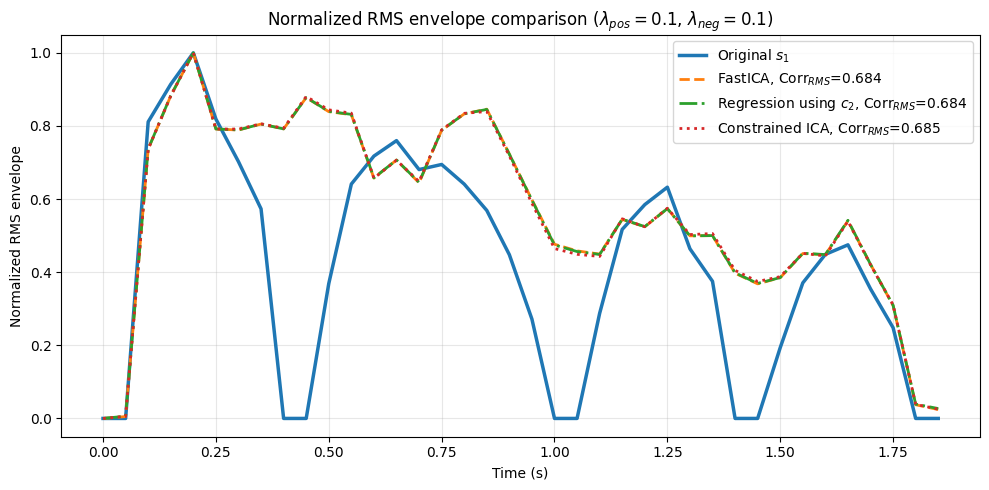
\includegraphics[width=\linewidth,height=6cm]{figuras/comparison_beta_03_tau_5.png}
    }
    \caption{Comparison  of the RMS envelopes recovered by constrained ICA, regression and standard FastICA algorithms. Parameters were set to $\sigma=0.1$, $\beta=0.3$ and $\tau=\qty{5}{ms}$. Prior information about the signal does not significantly improve recovery if the delayed contribution interference is specifically addressed.}
    \label{fig:constrained_regression_ica_comparison_with_delayed_regression}
\end{figure}
However, if the exact delay is known, a modified version of linear regression can be applied. As shown in Figure~\ref{fig:constrained_regression_ica_comparison_with_delayed_regression}, this approach leads to a substantial improvement over the non-delayed regression method. Nevertheless, \uline{this result is only possible because the delay is known} (in this case \qty{5}{ms}). In a real scenario, where only an approximate range may be available (\qtyrange{2}{10}{ms} for example) and the delay may take non-integer values, the separation quality would likely decrease considerably. 

\begin{figure}[H]
    \centering
    \makebox[\textwidth][c]{%
        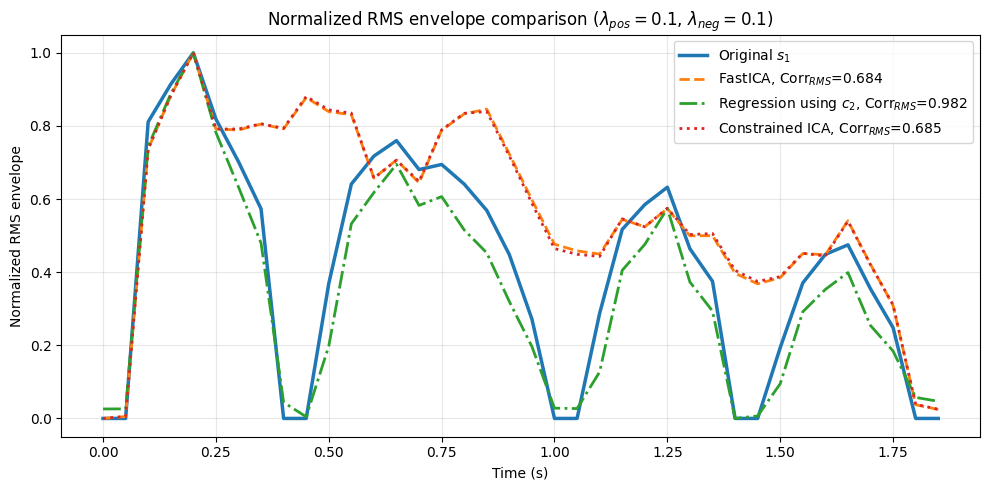
\includegraphics[width=\linewidth]{figuras/comparison_beta_05_tau_5_with_delayed_regression.png}
    }
    \caption{Comparison  of the RMS envelopes recovered by constrained ICA, \textbf{modified regression} and standard FastICA algorithms. Parameters were set to $\sigma=0.1$, $\beta=0.3$ and $\tau=\qty{5}{ms}$. The delayed regression achieves an almost perfect reconstruction as it removes the delayed interference from $s_2$.}
    \label{fig:constrained_regression_ica_comparison}
\end{figure}

\subsection{Best use scenario}

When testing multiple scenarios to assess under which conditions constrained ICA can improve standard ICA, the most noticeable improvement is observed in the instantaneous mixture case with a high noise level ($\sigma=0.5$). Table \ref{tab:lambda_grid_corr} shows the values of $\operatorname{Corr}_{\mathrm{RMS}}$ obtained for different combinations of $\lambda_{\mathrm{pos}}$ and $\lambda_{\mathrm{neg}}$. The best result is achieved when $\lambda_{\mathrm{pos}}=\lambda_{\mathrm{neg}}=0.05$, resulting in an improvement of approximately $4\%$ with respect to standard ICA.

This may indicate that the reference signals provide valuable information when the noise level is high and there is no significant delayed contribution from $s_2$.

\begin{table}[H]
\centering
\resizebox{\textwidth}{!}{
\begin{tabular}{c|ccccccccc}
\hline
$\lambda_{pos} \backslash \lambda_{neg}$ 
& 0.00 & $\mathbf{0.05}$ & 0.10 & 0.20 & 0.50 & 1.00 & 2.00 & 5.00  \\
\hline
0.00 & 0.6638 & 0.7019 & 0.7026 & 0.7025 & 0.7020 & 0.7018 & 0.7016 & 0.7016  \\
$\mathbf{0.05}$ & 0.6440 & $\mathbf{0.7026}$ & 0.7026 & 0.7024 & 0.7020 & 0.7018 & 0.7016 & 0.7016  \\
0.10 & 0.6921 & 0.6971 & 0.7025 & 0.7023 & 0.7020 & 0.7018 & 0.7016 & 0.7016  \\
0.20 & 0.6987 & 0.6995 & 0.6999 & 0.7021 & 0.7019 & 0.7017 & 0.7016 & 0.7016  \\
0.50 & 0.7007 & 0.7008 & 0.7008 & 0.7009 & 0.7018 & 0.7017 & 0.7016 & 0.7015  \\
1.00 & 0.7011 & 0.7011 & 0.7012 & 0.7012 & 0.7013 & 0.7017 & 0.7016 & 0.7015  \\
2.00 & 0.7013 & 0.7013 & 0.7013 & 0.7013 & 0.7014 & 0.7014 & 0.7015 & 0.7015  \\
5.00 & 0.7014 & 0.7014 & 0.7014 & 0.7014 & 0.7014 & 0.7014 & 0.7015 & 0.2473  \\

\hline
\end{tabular}
}
\caption{RMS correlation values for different combinations of $\lambda_{pos}$ and $\lambda_{neg}$. Parameters set to $\beta=0.5,\sigma=0.5,\tau=0$ms.}
\label{tab:lambda_grid_corr}
\end{table}


However, this slight improvement does not solve the main limitations of FastICA in the recovery of the RMS envelope. Figure \ref{fig:constrained_regression_ica_comparison2} illustrates the RMS envelope estimates retrieved by the three algorithms. Although constrained ICA follows the original envelope trends more accurately in some regions, noise artifacts still introduce some artificial peaks in the estimated signal.
\begin{figure}[H]
    \centering
    \makebox[\textwidth][c]{
        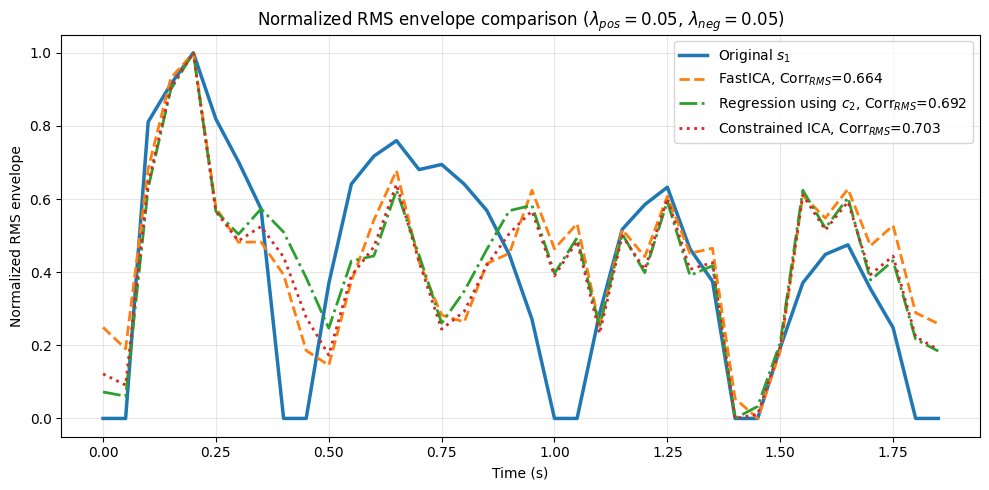
\includegraphics[width=\linewidth, height=6.5cm]{figuras/comparison_beta_05_tau_0.png}
    }
    \caption{Comparison  of the RMS envelopes recovered by constrained ICA, regression and standard FastICA algorithms. Parameters were set to $\sigma=0.5$, $\beta=0.3$ and $\tau=\qty{0}{ms}$. Results indicate that prior information may help in strong noise scenarios, but there is a limitation due to weak source scenario.}
    \label{fig:constrained_regression_ica_comparison2}
\end{figure}

\subsection{Constrained ICA Experiments Conclusion}

Overall, in the cases where standard FastICA does not perform optimally, adding prior information about the structure and behavior of the signals can only provide a slight improvement. However, the references used in these constrained ICA experiments are binary activation masks, since in real-world scenarios the true RMS envelope of the target signal would not be available ( it is precisely the signal that must be recovered). 

Additionally, using $c_2$ as an approximate reference of $s_2$ does not provide a significant improvement when $s_1$ remains clearly weak, both in the mixing matrix and in terms of variance. This suggests that, even though reference information can help guide the separation process, it does not fully overcome the major limitation imposed by the weak-source scenario.

A possible scenario where this algorithm could provide a more significant improvement over baseline ICA is a higher dimensional setting with several more channels and more sources. In the two source scenario case considered in this thesis, once one component is identified (often $s_2$ due to dominance), the remaining component is strongly dependent on orthogonality. However, when multiple sources are present, there are multiple possible orthogonal directions and ICA may have more difficulty selecting components. In that case, reference  constraints could help the algorithm towards the desired source. Nevertheless, this scenario is outside the scope presented on this thesis.